\paragraph{Reviewing an answer once.}
At $N=8$, on MATH-500, the two AceMath reward models score 86.69\% and 85.48\% in expectation over subsets. The archive contains 32,000 eligible responses and 7,978 question--answer units. With error-free reveals, the contrast order certifies the 1.21-point advantage after 437 answer judgments. The same priority applied to response-specific grades takes 11,942 judgments. Grouping by answer still helps without changing the priority to the contrast: pooling likely winners from the two systems requires 870 answer judgments (Table~\ref{tab:eight}). The two efficiencies arise from different operations, sharing grades between responses and canceling the probability that both systems assign to an answer.

\begin{table}[htbp]\centering\small
\caption{Audits at $N=8$. Gap is A minus B in percentage points. Checks count reveals until the sign is certified with $e=0$. Response and answer use absolute mass difference. Pool uses the larger winner mass on answer units. Radius is the smallest number of complete answer grades that could erase the lead.}\label{tab:eight}
\begin{tabular}{lrrrrrrr}\toprule
 & & & & \multicolumn{3}{c}{Checks to certify sign} & \\
Collection & Tasks & Answers & Gap & Response & Pool & Answer & Radius\\\midrule
\rowinput at_eight.tex
\bottomrule\end{tabular}
\end{table}

The initial MATH-500 answer-level gap width is 11.28 points. After reviewing 797 answers it is 0.78 points under contrast priority, 2.76 under pooled priority and 10.15 in expectation under uniform ordering. Allowing five errors in these 797 reviews still puts the gap between 0.21 and 2.10 points. In contrast, after revealing every Gaokao answer, even the sign at $N=8$ cannot be certified if five reviews might be wrong. Its complete-label radius is four. MMLU STEM requires 250 adverse changes at the same budget. These are sensitivity thresholds for mathematical answer grades.

\begin{figure}[htbp]\centering
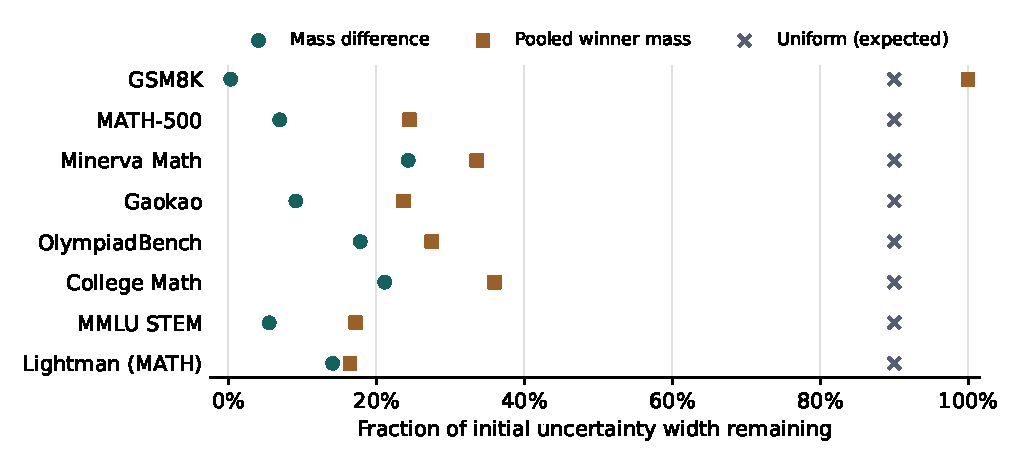
\includegraphics[width=.94\linewidth]{widths.pdf}
\caption{Residual answer-level uncertainty after reviewing $\lfloor 0.1m\rfloor$ of $m$ answers at $N=8$ with $e=0$. Each row is normalized by its own initial width. Uniform uses the exact expected width.}\label{fig:width}
\end{figure}

\paragraph{A second verifier family at a larger search depth.}
The Lightman release supplies 815,632 eligible scored responses for 500 problems, out of 930,000 generation slots. At $N=1{,}860$ we recover the published 78.2\% process-verifier and 72.4\% outcome-verifier accuracies. The target can be certified after 245 answer-unit checks under the first-occurrence grading convention. At $N=8$, it takes 20,356 such checks for a 0.69-point lead, and six adverse grade changes can erase it. At the full pool the lead rises to 5.80 points and the radius rises to 29. Thus the fall in Minerva's radius with increasing $N$ is not universal.

All 8,987 AceMath problem pools had consistent published grades within the declared answer units. There was one mixed-grade group among 94,816 Lightman units. It contained 67 responses. Choosing either shared binary grade can move the gap by at most 0.0014 points at $N=8$, 0.0015 at $N=32$ and 0.20 at $N=1{,}860$. The aggregate response-level gains using the original grades are 0.693, 2.078 and 5.800 points respectively. The answer-level checks for this release are conditional on the chosen resolution. Pooling without inspecting that assumption would conceal the inconsistency.

\paragraph{Generation budget and review reliability.}
On Gaokao the fully graded uniform-tie comparison changes from $+0.78$ points at $N=8$ to $-0.32$ at $N=32$ and $-1.04$ at $N=64$. Two adverse answer-grade changes suffice to erase the middle comparison. On Minerva Math the advantage grows from 3.13 to 4.78 points between $N=8$ and 64, while its radius falls from 23 to 13. Higher confidence in the ordering under missing labels can coexist with greater sensitivity to individual grades: a maximum over more draws can concentrate selection mass on fewer answers.

\begin{table}[htbp]\centering\scriptsize
\caption{Effect of generation budget on each fixed pool. Columns within each block use $N=8,32,M$. $M=64$ in AceMath and 1,860 in Lightman. Counts use exact answers and contrast priority.}\label{tab:scaling}
\begin{tabular}{lrrr rrr rrr}\toprule
&\multicolumn{3}{c}{Gap (points)}&\multicolumn{3}{c}{Checks to certify}&\multicolumn{3}{c}{Erasure radius}\\
Collection & 8 & 32 & Full & 8 & 32 & Full & 8 & 32 & Full\\\midrule
\rowinput scaling.tex
\bottomrule\end{tabular}
\end{table}

\paragraph{When adjudication is worth its cost.}
At $N=8$ on MATH-500, give an auditor 797 credits, set $e=5$, and charge five credits for reliable adjudication. Spending all credits on ordinary review gives a worst-transcript gap width of 1.96 points. Spending them exclusively on adjudication gives 5.30 points. The minimax design uses 23 reliable and 682 ordinary checks for a worst-case width of 1.52 points. At a smaller budget of 79 credits, the minimizer uses ordinary review alone. On GSM8K at $N=8$ with a 10\% budget and the same costs, the corresponding mixed width is 0.17 points against 0.52 and 0.51 points for the single-tier options. The economic premise is illustrative. The archive permits computation of the design for other costs before a reviewer is assigned.


\paragraph{Sensitivity to tie priority.}
The Gaokao reversal prompted a follow-up check on every subject. Within each tied score block, placing correct candidates first gives that verifier its best feasible value, and putting them last gives its worst. Subtract opposite extremes for the two verifiers to bound the gap over independently chosen tie priorities. This uses complete labels only to measure sensitivity. For Gaokao the interval is $[+0.73,+0.83]$ points at $N=8$, $[-0.45,-0.19]$ at 32 and $[-1.30,-0.78]$ at 64. Every such policy preserves the reversal on these fixed grades. The four-label erasure radius at 64 addresses a different perturbation, namely changing grades under the declared uniform-tie policy.

\paragraph{If solving one problem settles several answers.}
As a second follow-up, charge one check for adjudicating all answer units of a question. Its interval then collapses by $\sum_{i\in q}|d_i|$, so review questions in descending order of that sum. For complete grades, allow arbitrary changes within an affected question. The greatest loss for that question is its observed, winner-oriented contribution minus its lowest feasible contribution. Sorting these losses gives the minimum number of affected questions needed to erase the lead. At $N=8$ on AceMath MATH-500, 79 complete question checks certify the sign and adverse changes concentrated in six questions can erase it. On Gaokao the counts are 112 and two. At $N=32$ on Gaokao, changes within one question suffice. The calculation allows multiple changed judgments per problem. It does not assume that all those changes follow from substituting one valid answer key.
